\begin{figure}[p]
\centering
\captionsetup{justification=raggedright,labelsep=none,singlelinecheck=false,labelformat=boldlabel}
\caption[Sequential changes in out-of-sample RMSE relative to HAR.]{\footnotesize \textbf{: Sequential changes in out-of-sample RMSE relative to HAR.} Each column considers one extension of HARX. The bars first add exogenous covariates, then the indicated model extension, and finally the equal-weighted forecast combination. Positive changes represent lower RMSE. These arithmetic comparisons do not identify causal contributions.}
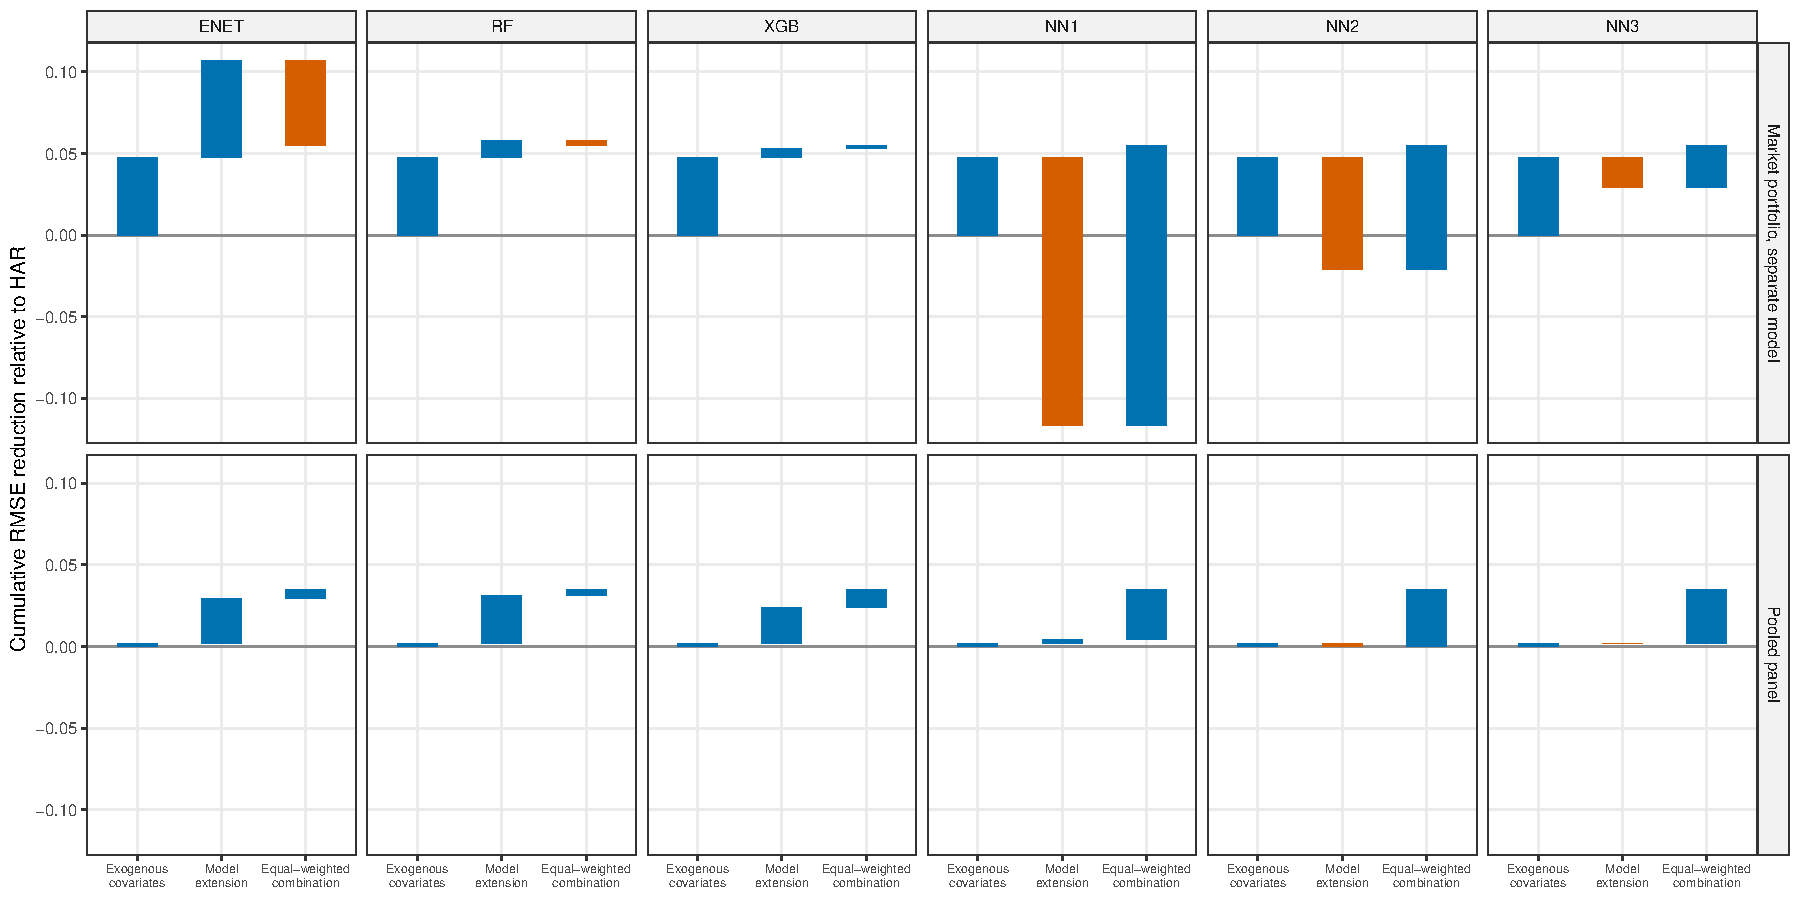
\includegraphics[width=\linewidth,height=0.78\textheight,keepaspectratio]{results_v3/1986/internet_appendix/sequential_waterfall.pdf}
\label{fig:rv-sequential_waterfall}
\end{figure}
